%% This is an example first chapter.  You should put chapter/appendix that you
%% write into a separate file, and add a line \include{yourfilename} to
%% main.tex, where `yourfilename.tex' is the name of the chapter/appendix file.
%% You can process specific files by typing their names in at the 
%% \files=
%% prompt when you run the file main.tex through LaTeX.
\chapter{Background and Related Work}
\section{Computer Musical Terminology}

\subsection{OMR}
OMR, or Optical Music Recognition, is method of recognizing the characters on scanned sheet music or printed scores and interpreting them into a digital form. OMR is great for large-scale fast digitization of scores. However, the current state-of-the-art of OMR leaves much room for improvement \cite{rebelo}. 

\subsection{MIDI}
MIDI is the protocol with which electronic instruments and computers can communicate with each other. Many people associate MIDI with an idea of low-quality computer music, but it is just an instruction-like protocol, not actually an audio recording. At the basic level, MIDI messages encode notes with note-on, note-off times, and a numbers that corresponds to their frequencies. A piece of music can be encoded in MIDI as a sequence of notes. On the other hand, MIDI files contain sequences of MIDI protocol events time-stamped for playback in a certain order.

\section{Non-musical Work in Sequence Alignment}
It is far easier to understand sequence alignment in a non-musical context (here the context is plain string alignment), understand the rules and assumptions made in the non-musical context, generalize them, and then recreate music-specific rules and assumptions. 

Readers familiar with the canonical representation of the string alignment problem as a dynamic programming matrix can skip this section. 

\subsection{An Overview of Sequence Alignment}
Sequence alignment in bioinformatics is an application of well-studied problem. In this field, researchers want to identify similar regions of DNA, RNA, or protein sequences to study functional, structural, or evolutionary relationships between the two sequences.

\begin{figure}[!ht]

\centering
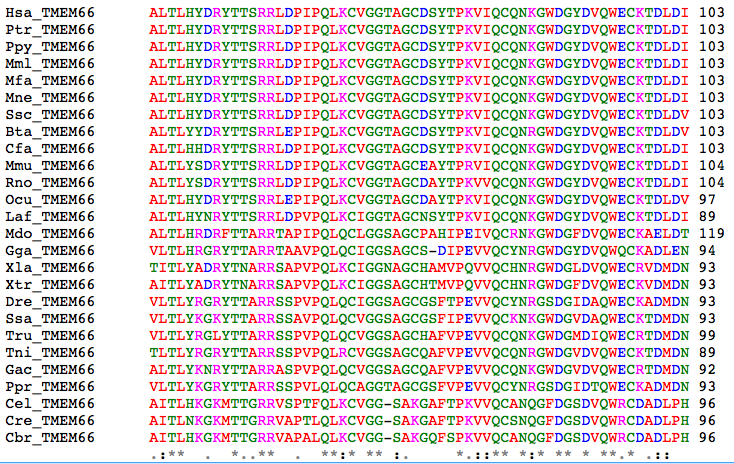
\includegraphics[scale=.5]{proteinalign}
\caption[An example of protein alignment] {An example of protein alignment }\cite{proteins}
\end{figure}

There are various computational algorithms that can be used to solve sequence alignment including slower but more accurate dynamic programming algorithms and faster but less accurate probabilistic or heuristic-based algorithms. In my work, it makes more sense to use the slower but more accurate methods, as our datasets are not so large and small mistakes that might be permissible to overlook in larger data could be much more egregious in smaller contexts.

The specific algorithm chosen to implement for solving the musical sequence alignment problem is a version of the Needleman-Wunsch dynamic programming algorithm for global sequence alignment \cite{needleman}. \footnote{This algorithm has a history of multiple invention. Needleman-Wunsch was first published in the context of protein alignment in bioinformatics. People with a more theoretical computer science bent might know the same algorithm by a different name, Wagner-Fisher.} 

At a high level, the Needleman-Wunsch algorithm and its family of dynamic programming sequence alignment algorithms calculate the edit distance between two sequences by producing a least-cost alignment of the sequences. An alignment is an assignment of pairwise characters and edit operations. Overall cost of an alignment (i.e. its \textbf{edit distance}) is determined by summing the individual costs of insertion, deletion, substitution, or no-change operations between pairwise characters in order to morph one sequence into the other. 

The next sections discuss coming up with edit distance calculations and then the method that Needleman-Wunsch uses to find the best alignment. 

\subsubsection{Edit Distance}

The term edit distance is a way of quantifying how dissimilar two sequences are from each other. If sequences are represented as an array of characters, then sequences can transform into each other through a series of insertion, deletion, substitution, and no-change operations, with each operation ``costing'' a certain amount. Edit distance is the smallest possible total cost associated with the transformation that is a series of operations that turns one sequence into another. As an example, consider the calculation of the edit distance between the two strings \textbf{MUSICAL} and \textbf{JUSTICE} that uses this series of operations for transforming \textbf{MUSICAL} into \textbf{JUSTICE}:

\begin{enumerate}
\item M $\rightarrow$  J (substitution)
\item $\epsilon \rightarrow$  T (insertion)
\item A $\rightarrow$  E (substitution)
\item L $\rightarrow  \epsilon$ (deletion)
\end{enumerate}


Note that implicitly excluded are all the no-change operations that look like this:
\begin{enumerate}
\item U $\rightarrow$  U (no-change)
\end{enumerate}

\begin{table}[!h]
\centering
\begin{tabular}{ll}
\textbf{Operation} & \textbf{Cost} \\
Insertion          & 1             \\
Deletion           & 1             \\
Substitution       & 1             \\
No-change          & 0            
\end{tabular}
\caption{Naive Operation Cost Function Table}
\label{tab:naivetable}
\end{table}
	
Figure \ref{best-alignment} corresponds to an alignment that looks like figure \ref{best-alignment}. The green pair of characters indicate an insertion operation, red is deletion, and purple is substitution. These colors are also used in the visualization of OMR/MIDI stream alignment. 

\begin{figure}[!h]
\centering
\begin{tabular}{lcccccccccccc}
seq1 & {\color[HTML]{6200C9} \textbf{M}} & \textbf{U} & \textbf{S} & {\color[HTML]{009901} \textbf{\_}} & \textbf{I} & \textbf{C} & {\color[HTML]{6200C9} \textbf{A}} & {\color[HTML]{9A0000} \textbf{L}}  & \textbf{} & \textbf{} & \textbf{} &  \\
seq2 & {\color[HTML]{6200C9} \textbf{J}} & \textbf{U} & \textbf{S} & {\color[HTML]{009901} \textbf{T}}  & \textbf{I} & \textbf{C} & {\color[HTML]{6200C9} \textbf{E}} & {\color[HTML]{9A0000} \textbf{\_}} & \textbf{} & \textbf{} & \textbf{} & 
\end{tabular}
\caption[Alignment of MUSICAL and JUSTICE]{The two strings have an edit distance of 4, because it requires four operations to completely morph one string into the other (discounting no-change operations).}
\label{best-alignment}
\end{figure}

One cost refinement that could be made is to slightly increase the cost of substitution. Since a substitution can be thought of as a consecutive insertion and deletion operation, but more compact, it should have a cost greater than that of a single insertion or deletion, but less than twice the cost of a single insertion/deletion. 

A slightly different cost function that assigns more cost to substitution changes could look like table \ref{tab:naivetable2}. Using this cost function, the edit distance of changing \textbf{MUSICAL} into \textbf{JUSTICE} is 5.
\begin{table}[!h]
\centering
\begin{tabular}{ll}
\textbf{Operation} & \textbf{Cost} \\
Insertion          & 1             \\
Deletion           & 1             \\
Substitution       & 1.5             \\
No-change          & 0            
\end{tabular}
\caption{Operation Cost Table With Costlier Substitutions}
\label{tab:naivetable2}
\end{table}

Yet another cost refinement is to give different subtypes of a single operation different weights. Consider if the application of trying to run a spell checker (one application of string alignment and correction algorithms) on a word that isn't recognized by the dictionary. In the particular spell check model, perhaps substitution of a vowel for a vowel isn't as costly as any other types of substitution, so vowel for vowel should only have a cost of 1.2. Using this new cost function, the new edit distance is 4.7.
\begin{table}[!h]
\centering
\begin{tabular}{ll}
\textbf{Operation}             & \textbf{Cost} \\
Insertion                      & 1             \\
Deletion                       & 1             \\
Substitution - vowel for vowel & 1.2           \\
Substitution - all others      & 1.5           \\
No-change                      & 0                
\end{tabular}
\caption{Operation Cost Table With Different Substitution Costs}
\label{my-label3}
\end{table}

Considerations such as these go into the creation of a musical sequence aligner as well. 
\subsubsection{Alignment}

Recall that the edit distance between two sequences is defined as the least-cost alignment. Figure \ref{badalign} shows a valid alignment, but it is certainly not the least-cost alignment, and therefore does not correspond to the edit distance between between the two sequences, as it requires four substitutions, one insertion, and one deletion.

\begin{figure}[!h]
\centering
\begin{tabular}{lcccccccccccc}
seq1 & {\color[HTML]{009901} \textbf{\_}} & {\color[HTML]{6200C9} \textbf{M}} & {\color[HTML]{6200C9} \textbf{U}} & {\color[HTML]{6200C9} \textbf{S}} & \textbf{I} & \textbf{C} & {\color[HTML]{6200C9} \textbf{A}} & {\color[HTML]{9A0000} \textbf{L}}  & \textbf{} & \textbf{} & \textbf{} &  \\
seq2 & {\color[HTML]{009901} \textbf{J}}  & {\color[HTML]{6200C9} \textbf{U}} & {\color[HTML]{6200C9} \textbf{S}} & {\color[HTML]{6200C9} \textbf{T}} & \textbf{I} & \textbf{C} & {\color[HTML]{6200C9} \textbf{E}} & {\color[HTML]{9A0000} \textbf{\_}} & \textbf{} & \textbf{} & \textbf{} & 
\end{tabular}
\caption{A bad alignment of MUSICAL and JUSTICE}
\label{badalign}
\end{figure}

If there are two sequences, of length $n$ and $m$, then they have $\binom{n+m}{m}$ possible alignments. Put into context, consider two melodies of 10 notes each. Naively aligning just the note pitches, there are 184,765 different possible alignments! Clearly this isn't scalable, which is why this piece of insight is important: A globally optimal alignment contains locally optimal alignments! This means that the computations of subproblems can be reused to solve larger problems. What follows from this piece of insight is that for two strings split at $(i, j)$, the best alignment is:

\begin{center}
best alignment of \texttt{string1}$[:i]$ and \texttt{string2}$[:j]$ 
$+$ best alignment of \texttt{string1}$[i:]$ and \texttt{string2}$[j:]$
\end{center}

\begin{figure}[!h]`
\centering
\begin{tabular}{lccccccc}
   & {\color[HTML]{333333} \textbf{}} & \multicolumn{2}{c}{{\color[HTML]{333333} $i$}}          & {\color[HTML]{333333} \textbf{}} & {\color[HTML]{333333} \textbf{}} & {\color[HTML]{333333} \textbf{}} & {\color[HTML]{333333} \textbf{}} \\
   & {\color[HTML]{333333} \textbf{}} & \multicolumn{2}{c}{{\color[HTML]{333333} $\downarrow$}} & {\color[HTML]{333333} \textbf{}} & {\color[HTML]{333333} \textbf{}} & {\color[HTML]{333333} \textbf{}} & {\color[HTML]{333333} \textbf{}} \\
\texttt{seq1} & \textbf{M}                       & \textbf{U}                  & \textbf{S}                & \textbf{I}                       & \textbf{C}                       & \textbf{A}                       & \textbf{L}                       \\
\texttt{seq2} & \textbf{J}                       & \textbf{U}                  & \textbf{S}                & \textbf{T}                       & \textbf{I}                       & \textbf{C}                       & \textbf{E}                       \\
   &                                  &                             &                           &                                  & \multicolumn{2}{c}{$\uparrow$}                                      &                                  \\
   &                                  &                             &                           &                                  & \multicolumn{2}{c}{$j$}                                             &                                 
\end{tabular}
\caption{The alignment of MUSICAL split at \textit{i} and JUSTICE split at \textit{j}}
\label{indexed musical and justice}
\end{figure}

If all the possible alignment subproblems are kept track of, it is possible to recursively build an optimal solution using the answers from the subproblems. One way to represent this is with a scoring matrix indexed by $i$ and $j$. For the problem of aligning \textbf{MUSICAL} and \textbf{JUSTICE}, the setup would look something like in figure \ref{alignsetup} 


\begin{figure}[!h]
\centering
\begin{tabular}{lllllllll}
                                & \multicolumn{1}{c}{\textbf{-}} & \textbf{J}            & \textbf{U}            & \textbf{S}            & \textbf{T}            & \textbf{I}            & \textbf{C}            & \textbf{E}            \\ \cline{2-9} 
\multicolumn{1}{c|}{\textbf{-}} & \multicolumn{1}{l|}{}          & \multicolumn{1}{l|}{} & \multicolumn{1}{l|}{} & \multicolumn{1}{l|}{} & \multicolumn{1}{l|}{} & \multicolumn{1}{l|}{} & \multicolumn{1}{l|}{} & \multicolumn{1}{l|}{} \\ \cline{2-9} 
\multicolumn{1}{l|}{\textbf{M}} & \multicolumn{1}{l|}{}          & \multicolumn{1}{l|}{} & \multicolumn{1}{l|}{} & \multicolumn{1}{l|}{} & \multicolumn{1}{l|}{} & \multicolumn{1}{l|}{} & \multicolumn{1}{l|}{} & \multicolumn{1}{l|}{} \\ \cline{2-9} 
\multicolumn{1}{l|}{\textbf{U}} & \multicolumn{1}{l|}{}          & \multicolumn{1}{l|}{} & \multicolumn{1}{l|}{} & \multicolumn{1}{l|}{} & \multicolumn{1}{l|}{} & \multicolumn{1}{l|}{} & \multicolumn{1}{l|}{} & \multicolumn{1}{l|}{} \\ \cline{2-9} 
\multicolumn{1}{l|}{\textbf{S}} & \multicolumn{1}{l|}{}          & \multicolumn{1}{l|}{} & \multicolumn{1}{l|}{} & \multicolumn{1}{l|}{} & \multicolumn{1}{l|}{} & \multicolumn{1}{l|}{} & \multicolumn{1}{l|}{} & \multicolumn{1}{l|}{} \\ \cline{2-9} 
\multicolumn{1}{l|}{\textbf{I}} & \multicolumn{1}{l|}{}          & \multicolumn{1}{l|}{} & \multicolumn{1}{l|}{} & \multicolumn{1}{l|}{} & \multicolumn{1}{l|}{} & \multicolumn{1}{l|}{} & \multicolumn{1}{l|}{} & \multicolumn{1}{l|}{} \\ \cline{2-9} 
\multicolumn{1}{l|}{\textbf{C}} & \multicolumn{1}{l|}{}          & \multicolumn{1}{l|}{} & \multicolumn{1}{l|}{} & \multicolumn{1}{l|}{} & \multicolumn{1}{l|}{} & \multicolumn{1}{l|}{} & \multicolumn{1}{l|}{} & \multicolumn{1}{l|}{} \\ \cline{2-9} 
\multicolumn{1}{l|}{\textbf{A}} & \multicolumn{1}{l|}{}          & \multicolumn{1}{l|}{} & \multicolumn{1}{l|}{} & \multicolumn{1}{l|}{} & \multicolumn{1}{l|}{} & \multicolumn{1}{l|}{} & \multicolumn{1}{l|}{} & \multicolumn{1}{l|}{} \\ \cline{2-9} 
\multicolumn{1}{l|}{\textbf{L}}   & \multicolumn{1}{l|}{}          & \multicolumn{1}{l|}{} & \multicolumn{1}{l|}{} & \multicolumn{1}{l|}{} & \multicolumn{1}{l|}{} & \multicolumn{1}{l|}{} & \multicolumn{1}{l|}{} & \multicolumn{1}{l|}{} \\ \cline{2-9} 
\end{tabular}
\caption{Initial distance matrix setup for aligning MUSICAL and JUSTICE}
\label{alignsetup}
\end{figure}

Recall that the problem has been defined in three different ways:
\begin{enumerate}
\item Aligning \textbf{MUSICAL} and \textbf{JUSTICE}
\item Finding the edit distance between \textbf{MUSICAL} and \textbf{JUSTICE}
\item Finding a series of operations that transforms \textbf{MUSICAL} into \textbf{JUSTICE}
\end{enumerate}

All of these problem definitions are (almost) one and the same. Calculating the edit distance will also provide a good alignment of the two words and a good alignment necessitates a series of character change operations. It is important to know that (3) has an implicit directionality built into the problem statement. It won't always be the case that alignments and transformations are symmetric (i.e. cost the same and have the same series of operations), but having a simple cost operation functions, such as in tables \ref{tab:naivetable} and \ref{tab:naivetable2}, will make such problems symmetric. 

In this particular sample problem, it is always the case that the word \textbf{MUSICAL} is  transformed into another word, \textbf{JUSTICE}. In this particular context, OMR sequences are transformed into MIDI sequences. 

After the scoring matrix is set up, it is populated with initial values: 
\begin{enumerate}
\item 0 in $(0,0)$
\item $i-1 \cdot insertion cost$ for $i$ in $(i, 0)$ (this is the first column) 
\item $j-1 \cdot deletion cost$ for $j$ in $(0, j)$ (this is the first column) 
\end{enumerate}
In reading a scoring matrix setup like this, insertions are vertical movements, deletions are horizontal movements, and substitutions are diagonal. 
After setting up the initial matrix, all of the remaining slots are filled in using this update rule:


\begin{equation*}
\begin{split}
\text{D[i][j]} = &  \text{min \{ }\\
& \text{D[i-1][j] + insCost (the cell above),} \\
& \text{D[i][j-1] + delCost (the cell to the left),} \\
& \text{D[i-1][j-1] + subCost (the cell diagonal, up and to the left)} \\
\text{\}}
\end{split}
\end{equation*}


\section{Turning Sequence Alignment into a Musical Problem}
Finding the edit distance of a musical sequence as opposed to a string of ASCII characters is a little trickier. First, there isn't an intuitive ``space'' of music elements the way that there is a ``space'' of all characters. Second, even after identifying the musical elements, there isn't an intuitive metric of distance between elements. For example, how would the distance between an A\# quarter note in the 4th octave and a B quarter note in the 4th octave compare with an A\# eighth note in the 4th octave and an A\# quarter note in the 4th octave?

By massaging musical sequences into string-like objects, it becomes easier to see how techniques in string alignment can be applied to musical sequence alignment. The questions and answers posed below help identify parallels between strings and musical sequences. 

\begin{itemize}
\item What are sequences are and what makes them up?: musical sequences can be thought of as an ordering of notes, rests, and chords.
\item What is the space that sequences occupy?: This question can roughly be approximated as, what are the important properties of notes, rests, chords? Some immediate answers are pitch, duration, offset.
\item What is an appropriate metric for distance?: In the previous section there were multiple different substitution functions. What kind of and how many ways are there to calculate distance between musical elements? Perhaps representing a musical element as a tuple of numbers, (pitch, duration, offset) gives us points in space that we can calculate distance. 
\end {itemize}

Once musical sequences can be represented in string-like formats, we can perform string operations on them. The next chapter discusses related work by others who have explored some part of this musical sequence alignment question as well as my own previous work that relates to this thesis. 
